\documentclass[11pt]{article}
\usepackage[margin=1in]{geometry}
\usepackage{booktabs}
\usepackage{enumitem}
\usepackage{hyperref}
\usepackage[T1]{fontenc}
\usepackage{textcomp}
\usepackage{float}
\usepackage{tikz}
\usetikzlibrary{arrows.meta, positioning}

\title{ICIS-Air Data Structure}
\author{}
\date{}

\begin{document}
\maketitle

\section{Overview}

The EPA's Integrated Compliance Information System for Air (ICIS-Air) provides 10 downloadable tables covering the universe of Clean Air Act regulated facilities. All tables share \texttt{PGM\_SYS\_ID} as the primary join key, which identifies a regulated facility. A secondary identifier, \texttt{REGISTRY\_ID}, links to the Facility Registry Service (FRS) and identifies a physical site. Multiple \texttt{PGM\_SYS\_ID}s can map to one \texttt{REGISTRY\_ID} when a single site has multiple separately regulated facilities.

\section{Table Inventory}

\begin{table}[H]
\centering
\begin{tabular}{llrl}
\toprule
Table & Grain & Rows & Key Fields \\
\midrule
FACILITIES & 1 row per facility & 279,211 & Static characteristics \\
PROGRAMS & Facility $\times$ program & 456,601 & Program enrollment, dates \\
PROGRAM\_SUBPARTS & Facility $\times$ subpart & 190,570 & MACT/NSPS subpart codes \\
POLLUTANTS & Facility $\times$ pollutant & 976,479 & Regulated pollutants \\
FCES\_PCES & Evaluation event & 1,802,044 & Inspection type, date \\
VIOLATION\_HISTORY & Violation event & 101,147 & HPV/FRV, dates, resolution \\
FORMAL\_ACTIONS & Formal enforcement event & 105,656 & Action type, penalty \\
INFORMAL\_ACTIONS & Informal enforcement event & 336,410 & NOV/warning, date \\
STACK\_TESTS & Stack test event & 646,332 & Pass/fail, pollutants \\
TITLEV\_CERTS & Certification event & 2,563,435 & Deviation flag \\
\bottomrule
\end{tabular}
\caption{ICIS-Air tables. All tables key on \texttt{PGM\_SYS\_ID}.}
\end{table}

\section{How the Tables Connect}

\begin{figure}[H]
\centering
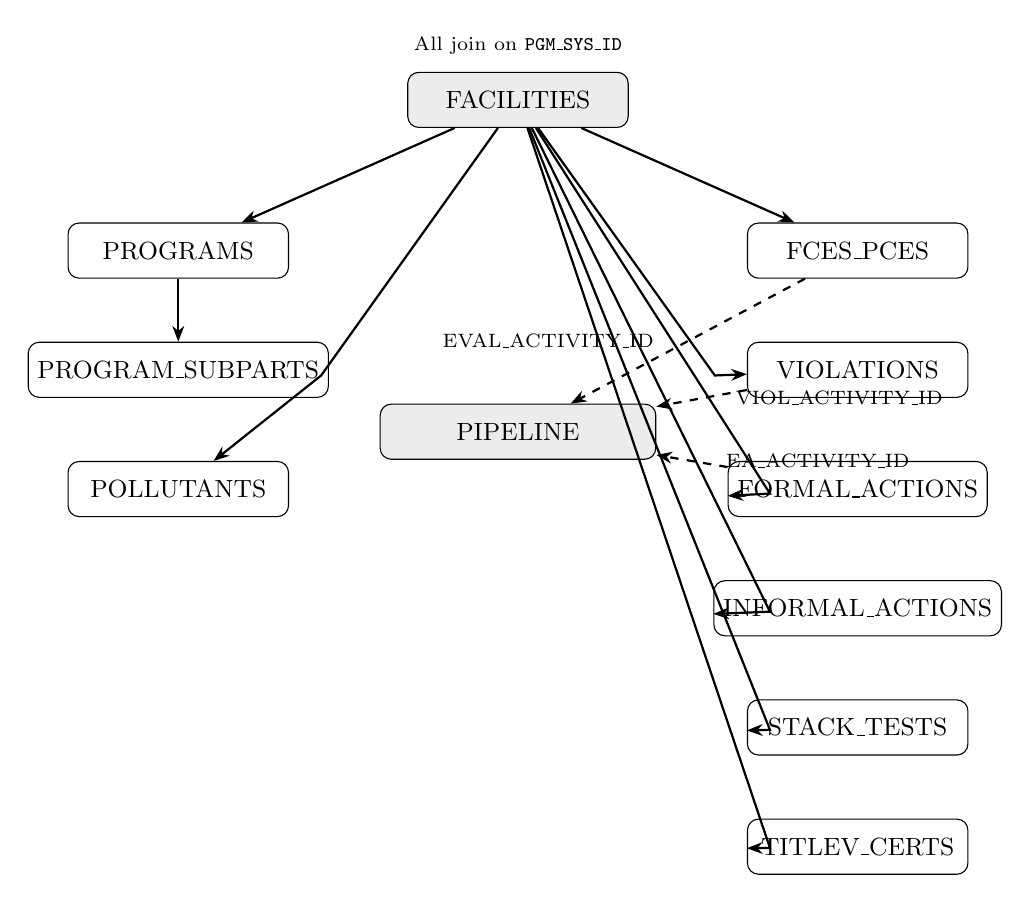
\begin{tikzpicture}[
    node distance=1.2cm and 2.5cm,
    every node/.style={draw, rounded corners, minimum width=2.8cm, minimum height=0.7cm, font=\small},
    arrow/.style={-{Stealth[length=2mm]}, thick},
    label/.style={font=\scriptsize, draw=none, minimum width=0, minimum height=0}
  ]
  % Master table
  \node (fac) [fill=gray!15] {FACILITIES};

  % Static descriptors (left branch)
  \node (prog) [below left=1.2cm and 1.5cm of fac] {PROGRAMS};
  \node (sub)  [below=0.8cm of prog] {PROGRAM\_SUBPARTS};
  \node (poll) [below=0.8cm of sub] {POLLUTANTS};

  % Event tables (right branch)
  \node (eval) [below right=1.2cm and 1.5cm of fac] {FCES\_PCES};
  \node (viol) [below=0.8cm of eval] {VIOLATIONS};
  \node (form) [below=0.8cm of viol] {FORMAL\_ACTIONS};
  \node (info) [below=0.8cm of form] {INFORMAL\_ACTIONS};
  \node (stk)  [below=0.8cm of info] {STACK\_TESTS};
  \node (cert) [below=0.8cm of stk] {TITLEV\_CERTS};

  % Pipeline
  \node (pipe) [below=3.5cm of fac, fill=gray!15, minimum width=3.5cm] {PIPELINE};

  % Arrows from master
  \draw[arrow] (fac) -- (prog);
  \draw[arrow] (fac) -- (eval);

  % Static chain
  \draw[arrow] (prog) -- (sub);
  \draw[arrow] (fac) -- +(-2.5,-3.5) -- (poll);

  % Event arrows from master
  \draw[arrow] (fac) -- +(2.5,-3.5) -- (viol);
  \draw[arrow] (fac) -- +(3.2,-5) -- (form);
  \draw[arrow] (fac) -- +(3.2,-6.5) -- (info);
  \draw[arrow] (fac) -- +(3.2,-8) -- (stk);
  \draw[arrow] (fac) -- +(3.2,-9.5) -- (cert);

  % Pipeline connections
  \draw[arrow, dashed] (viol) -- (pipe) node[label, midway, right, xshift=3mm] {VIOL\_ACTIVITY\_ID};
  \draw[arrow, dashed] (form) -- (pipe) node[label, midway, right, xshift=3mm] {EA\_ACTIVITY\_ID};
  \draw[arrow, dashed] (eval) -- (pipe) node[label, midway, left, xshift=-3mm] {EVAL\_ACTIVITY\_ID};

  % Join key label
  \node[label, above=0.1cm of fac, draw=none] {All join on \texttt{PGM\_SYS\_ID}};
\end{tikzpicture}
\caption{Table relationships. Solid arrows: join on \texttt{PGM\_SYS\_ID}. Dashed arrows: the Pipeline pre-joins violations, evaluations, and enforcement actions via \texttt{ACTIVITY\_ID}.}
\end{figure}

\subsection*{Two types of tables}

\textbf{Static tables} describe time-invariant (or slowly changing) characteristics of a facility:

\begin{itemize}[nosep]
  \item \textbf{FACILITIES}: master roster. One row per \texttt{PGM\_SYS\_ID}. Contains location, industry (NAICS/SIC), emissions classification (major/minor), and operating status.
  \item \textbf{PROGRAMS}: which CAA programs a facility is enrolled in (CAATVP = Title V, CAASIP = SIP, CAAMACT = MACT, etc.) with enrollment dates. Multiple rows per facility---one per program.
  \item \textbf{PROGRAM\_SUBPARTS}: regulatory subpart detail within each program (e.g., which MACT subpart applies). Joins to PROGRAMS on \texttt{PGM\_SYS\_ID} + \texttt{PROGRAM\_CODE}.
  \item \textbf{POLLUTANTS}: which pollutants a facility is regulated for. Multiple rows per facility---one per pollutant.
\end{itemize}

\textbf{Event tables} record time-stamped regulatory interactions:

\begin{itemize}[nosep]
  \item \textbf{FCES\_PCES}: compliance evaluations (inspections). Each row is one evaluation event with an \texttt{ACTIVITY\_ID}, type code (FCE on-site = \texttt{FOO}, FCE off-site = \texttt{FFO}; 9 PCE codes), and date.
  \item \textbf{VIOLATION\_HISTORY}: discovered violations. Each row is one violation with type (HPV or FRV), determination date, and resolution date (if resolved).
  \item \textbf{FORMAL\_ACTIONS}: formal enforcement (administrative orders, judicial actions). Contains penalty amounts and settlement dates.
  \item \textbf{INFORMAL\_ACTIONS}: informal enforcement (notices of violation = \texttt{NOV}, warning letters = \texttt{DAWL}). Contains achieved date.
  \item \textbf{STACK\_TESTS}: emissions testing events with pass/fail status and pollutant codes.
  \item \textbf{TITLEV\_CERTS}: annual Title V compliance certifications. Contains \texttt{FACILITY\_RPT\_DEVIATION\_FLAG} (Y/N) indicating whether the facility self-reported deviations.
\end{itemize}

\subsection*{Cross-table linkages beyond PGM\_SYS\_ID}

The event tables each assign their own \texttt{ACTIVITY\_ID}, but these IDs are not shared across tables. A formal action's \texttt{ACTIVITY\_ID} does not appear in the violation table, and vice versa. The tables do not record which enforcement action responded to which violation, or which evaluation discovered which violation.

The \textbf{Pipeline} dataset (\texttt{PIPELINE\_CAA\_00\_COMPLETE.csv}) fills this gap by pre-joining violations to their linked evaluations and enforcement actions. It uses \texttt{VIOL\_ACTIVITY\_ID}, \texttt{EA\_ACTIVITY\_ID}, and \texttt{EVAL\_ACTIVITY\_ID} to create the linkage. See the Pipeline Brief for details.

\section{Key Relationships and Caveats}

\begin{enumerate}[nosep]
  \item \textbf{PGM\_SYS\_ID vs.\ REGISTRY\_ID}: \texttt{PGM\_SYS\_ID} identifies a regulated facility; \texttt{REGISTRY\_ID} identifies a physical site. Multiple \texttt{PGM\_SYS\_ID}s can therefore share one \texttt{REGISTRY\_ID} when a site contains separately regulated facilities.

  \item \textbf{No direct violation-to-enforcement link}: the individual ICIS-Air tables do not record which enforcement action responded to which violation. A facility with 3 violations and 2 formal actions in the same year has no table-level information about which actions addressed which violations. The Pipeline dataset provides this linkage.

  \item \textbf{Date field choice matters}: violations carry multiple date fields (\texttt{HPV\_DAYZERO\_DATE}, \texttt{EARLIEST\_FRV\_DETERM\_DATE}, pathway dates), so the choice of field affects which period an event is assigned to. Formal actions use \texttt{SETTLEMENT\_ENTERED\_DATE}, which may lag the initial filing by months or years.

  \item \textbf{Evaluation type codes are abbreviations}: FCE on-site = \texttt{FOO}, FCE off-site = \texttt{FFO}. PCE codes include \texttt{PCE}, \texttt{PFF}, \texttt{PFR}, \texttt{POC}, \texttt{POF}, \texttt{POI}, \texttt{POM}, \texttt{POR}, \texttt{POV}. These are not self-documenting; they are documented in EPA's ICIS-Air data dictionary.

  \item \textbf{Event tables are not mutually exclusive}: a single regulatory interaction can generate records in multiple tables. An FCE that discovers a violation that leads to a formal action with a penalty produces rows in FCES\_PCES, VIOLATION\_HISTORY, and FORMAL\_ACTIONS---so the same underlying interaction appears in several tables.

  \item \textbf{Certifications are Title V only}: \texttt{TITLEV\_CERTS} covers only Title V facilities. For non-Title V analyses, this table contributes nothing, and the self-reported deviation flag is unavailable.
\end{enumerate}

\end{document}
